
\chapter{2. Linear PDEs: a structured grid example}

We start with the Poisson problem because it is the right place to start.  Though it is a cliche in applied mathematics, in solving it we will use key parts of \PETSc: build a structured grid using a \PETSc \pDMDA, assemble a \pMat and some \pVecs in parallel on this grid, and solve in parallel using a \pKSP object.

\section{A Poisson problem on a square domain}

It is common to see the \emph{Laplacian}
    $$\grad^2 u = \Div(\grad u) = \frac{\partial^2 u}{\partial x^2} + \frac{\partial^2 u}{\partial y^2}$$
of a function $u(x,y)$ in a mathematical model.  The Laplacian almost always appears because the quantity $u$ is conserved, and from an assumption that the gradient $\grad u$ is, up to a coefficient, the flux of $u$ \citep{Ockendonetal2003}.  The divergence ``$\Div$'' arises from the connection between a flux integral over a closed surface and an integral over the interior of that surface, namely, from the divergence (Gauss) theorem (FIXME cite).

In the \emph{Poisson equation} the Laplacian of $u$ is equal to a known function.  We cannot just solve this one equation on a finite region, however.  We solve a \emph{Poisson problem} including boundary conditions, and the whole problem determines a solution which we will find (approximate) numerically.  Let $\mathcal{S}$ be the open unit square $(0,1)\times(0,1)$.  The following is our Poisson problem for this Chapter;  see Figure \ref{fig:unitsquare}:
\begin{marginfigure}
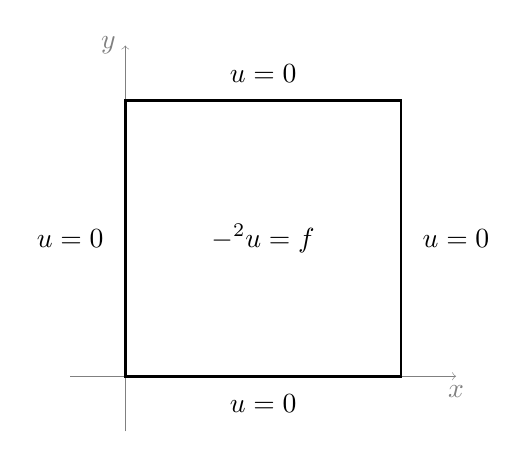
\begin{tikzpicture}[scale=3.5]
  \draw[->,gray,very thin] (-0.2,0.0) -- (1.2,0.0) node[below] {$x$};
  \draw[->,gray,very thin] (0.0,-0.2) -- (0.0,1.2) node[left] {$y$};
  \draw[line width=1.0pt] (0.0,0.0) -- (0.0,1.0) -- (1.0,1.0) -- (1.0,0.0) -- cycle;
  \node at (0.5,0.5) {$- \grad^2 u = f$};
  \node at (0.5,-0.1) {$u = 0$};
  \node at (0.5,1.1) {$u = 0$};
  \node at (-0.2,0.5) {$u = 0$};
  \node at (1.2,0.5) {$u = 0$};
\end{tikzpicture}
\caption{Our first, simple goal is to solve the Poisson equation on the unit square $\mathcal{S}$, with homogeneous Dirichlet boundary conditions.}
\label{fig:unitsquare}
\end{marginfigure}
\begin{align}
- \grad^2 u &= f \quad \text{ on } \mathcal{S}, \label{poissonsquare} \\
u &= 0 \quad \text{ on } \partial \mathcal{S}. \notag
\end{align}
The boundary of the unit square, denoted ``$\partial\mathcal{S}$'', is simply the union of four (closed) line segments.  The boundary conditions $u=0$ are called ``\emph{homogeneous Dirichlet}.''

The Poisson problem can model the distribution of temperature in a conducting object at steady state, the electrostatic potential, the equilibrium distribution from certain random walks, and many other other physical phenomena.  For example, in the context of heat conduction Fourier's law says $\bq = -k \grad u$, where $k$ is approximately constant if the variation in $u$ is not too large.  Conservation of energy for a solid says $c\rho \partial u/\partial t = - \Div\bq + f$ if $f$ describes a heat source within the domain.  At steady state ($\partial u/\partial t=0$) this equation becomes $0 = k \grad^2 u + f$, that is, Poisson's equation \eqref{poissonsquare}.  Holding the temperature fixed at zero along the boundary completes the problem.

For this chapter we will suppose that $f(x,y)$ is continuous and bounded on $\mathcal{S}$, so that we can compute its pointwise values.  With our homogeneous Dirichlet boundary conditions, and the assumptions on $f$, standard theory says that $u(x,y)$ exists and is continuous on the closed square $\overline{\mathcal{S}}$.\sidenote{One approach to showing this classical-existence fact starts by solving the problem \eqref{poissonsquare} by Fourier series!  Because $f$ itself is square-integrable, the Fourier coefficients $\hat f$ are square-integrable (Parseval's equality).  Because the Laplacian is elliptic and second-order, the coefficients $\hat u$ are square-integrable even when multiplied by the square of the frequency.  By a Cauchy-Schwarz argument, one then shows that the Fourier series for $u$ is the limit of a sequence of continuous functions on $\overline{\mathcal{S}}$ which converge uniformly.  (\emph{For a more abstract version see Theorem 6 in section 5.6 of \citet{Evans}.})}  Thus there is no ambiguity in the boundary condition ``$u=0$ on $\partial \mathcal{S}$,'' and furthermore we can sensibly discuss the pointwise values $u(x,y)$.

Without any boundary conditions, the Poisson equation $-\grad^2 u = f$ alone is not a well-posed problem because if $-\grad^2 u = f$ then also $-\grad^2(u+C)=f$ for any constant $C$; in fact there are these constant solutions and many, many more to the Laplace equation $-\grad^2 u = 0$ on $\mathcal{S}$.  With the Dirichlet boundary conditions in \eqref{poissonsquare}, the solution is unique if it exists.\sidenote{See Theorem 5 in section 2.2 of \citet{Evans} or subsection 5.2.1 of \citet{Ockendonetal2003}.}


\section{A finite difference method: the grid in parallel}

Because \eqref{poissonsquare} is a linear problem, finite-dimensional approximations of it are simply linear systems.  The finite-dimensional approximation in this Chapter comes from applying a \emph{finite difference} (FD) method.

To start our FD method we put a \emph{structured grid} of $MN$ points on the unit square, as in Figure \ref{fig:unitsquaregrid}, with spacing $h_x=1/(M-1)$ and $h_y=1/(N-1)$ in the two directions.  The grid locations are $x_i = i\, h_x$ and $y_j = j\, h_y$ for $i = 0,1,\dots,M-1$ and $j=0,1,\dots,N-1$.

\begin{marginfigure}
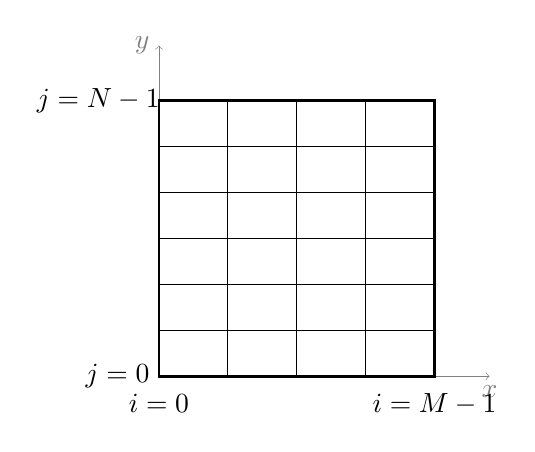
\begin{tikzpicture}[scale=3.5]
  \draw[->,gray,very thin] (0.0,0.0) -- (1.2,0.0) node[below] {$x$};
  \draw[->,gray,very thin] (0.0,0.0) -- (0.0,1.2) node[left] {$y$};
  \draw[line width=1.0pt] (0.0,0.0) -- (0.0,1.0) -- (1.0,1.0) -- (1.0,0.0) -- cycle;
  \node at (0.0,-0.1) {$i=0$};
  \node at (1.0,-0.1) {$i=M-1$};
  \node at (-0.15,0.0) {$j=0$};
  \node at (-0.22,1.0) {$j=N-1$};
  \draw[xstep=0.25,ystep=0.166667,black,thin] (0.0,0.0) grid (1.0,1.0);
\end{tikzpicture}
\caption{A grid on the unit square $\mathcal{S}$, with $M=5$ and $N=7$.}
\label{fig:unitsquaregrid}
\end{marginfigure}

The construction of such a two-dimensional (2D) grid, and the distribution of it across processors, is our first new idea from \PETSc beyond the basics in Chapter 1.  Consider these lines
\begin{Verbatim}[fontsize=\small]
  DM  da;
  DMDACreate2d(PETSC_COMM_WORLD,
               DM_BOUNDARY_NONE, DM_BOUNDARY_NONE, DMDA_STENCIL_STAR,
               -9,-9,PETSC_DECIDE,PETSC_DECIDE,1,1,NULL,NULL,
               &da);
  DMDASetUniformCoordinates(da,0.0,1.0,0.0,1.0,-1.0,-1.0);
\end{Verbatim}
\medskip\noindent
which create a \PETSc \pDM object\sidenote{``\pDM'' might stand for ``data management'', but perhaps ``distributed mesh'' is a better expansion.} for a grid like that shown in Figure \ref{fig:unitsquaregrid}.

A \pDM is an abstract type for describing the topology (i.e.~connectedness) of a grid, \emph{and} the way it is distributed across \MPI processes, \emph{and} the way each process's part of the grid can access its neighbors.  The specific variable \texttt{da} is above created to have type ``\pDMDA'', which is the subclass of \pDM s which are structured grids.  The above lines of code will appear in \texttt{c2poisson.c} below.  Supposing we call
\begin{Verbatim}[fontsize=\small]
  mpiexec -n 4 c2poisson -da_grid_x 5 -da_grid_y 7
\end{Verbatim}
\medskip\noindent
then a structured grid like that in Figure \ref{fig:unitsquaregrid} will be created, but with the parallel decomposition shown in Figure \ref{fig:unitsquaregridparallel}.  In fact, \PETSc itself can show the parallel layout by calling
\begin{Verbatim}[fontsize=\small]
  mpiexec -n 4 c2poisson -da_grid_x 5 -da_grid_y 7 -dm_view
\end{Verbatim}
\noindent
or
\begin{Verbatim}[fontsize=\small]
  mpiexec -n 4 c2poisson -da_grid_x 5 -da_grid_y 7 \
      -dm_view draw -draw_pause -1
\end{Verbatim}
\noindent
The latter version shows the grid graphically, and labels the nodes with the local order; use mouse clicks to cycle through the displays.

\begin{marginfigure}
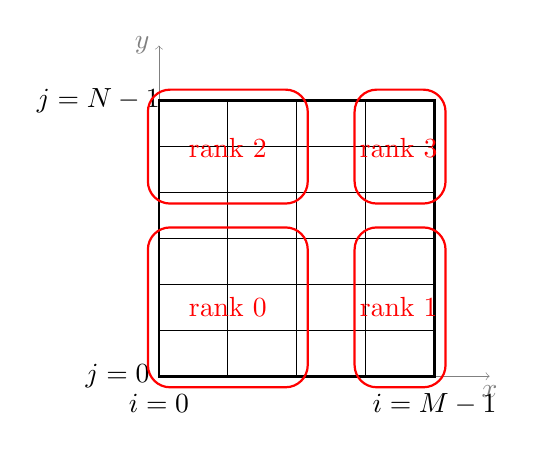
\begin{tikzpicture}[scale=3.5]
  \draw[->,gray,very thin] (0.0,0.0) -- (1.2,0.0) node[below] {$x$};
  \draw[->,gray,very thin] (0.0,0.0) -- (0.0,1.2) node[left] {$y$};
  \draw[line width=1.0pt] (0.0,0.0) -- (0.0,1.0) -- (1.0,1.0) -- (1.0,0.0) -- cycle;
  \node at (0.0,-0.1) {$i=0$};
  \node at (1.0,-0.1) {$i=M-1$};
  \node at (-0.15,0.0) {$j=0$};
  \node at (-0.22,1.0) {$j=N-1$};
  \draw[xstep=0.25,ystep=0.166667,black,thin] (0.0,0.0) grid (1.0,1.0);
  \draw[thick,rounded corners=8pt,color=red]
(-0.04,-0.04) -- (-0.04,0.54) -- (0.54,0.54) -- (0.54,-0.04) -- cycle;
  \node[color=red] at (0.25,0.25) {rank $0$};
  \draw[thick,rounded corners=8pt,color=red]
(0.71,-0.04) -- (0.71,0.54) -- (1.04,0.54) -- (1.04,-0.04) -- cycle;
  \node[color=red] at (0.87,0.25) {rank $1$};
  \draw[thick,rounded corners=8pt,color=red]
(-0.04,0.626667) -- (-0.04,1.04) -- (0.54,1.04) -- (0.54,0.62667) -- cycle;
  \node[color=red] at (0.25,0.83) {rank $2$};
  \draw[thick,rounded corners=8pt,color=red]
(0.71,0.626667) -- (0.71,1.04) -- (1.04,1.04) -- (1.04,0.626667) -- cycle;
  \node[color=red] at (0.87,0.83) {rank $3$};
\end{tikzpicture}
\caption{A grid on the unit square $\mathcal{S}$, with $M=5$ and $N=7$, distributed across four \MPI processes (i.e.~with \texttt{rank} $\in \{0,1,2,3\}$) automatically by \texttt{DMDACreate2d()}.}
\label{fig:unitsquaregridparallel}
\end{marginfigure}

The above command \texttt{DMDACreate2d()} creates the \pDMDA object as a 2D structured grid but a bit more explanation than that is needed.   The \PETSc manual pages description of that method is
\begin{Verbatim}[fontsize=\small]
DMDACreate2d(MPI_Comm comm, DMBoundaryType bx, DMBoundaryType by,
  DMDAStencilType stype, PetscInt M, PetscInt N, PetscInt m, PetscInt n,
  PetscInt dof, PetscInt s, const PetscInt lx[], const PetscInt ly[],
  DM *da)
\end{Verbatim}
where
\small
\begin{itemize}[align=left]
\item[\texttt{comm}]   MPI communicator \\
\item[\texttt{bx,by}]  type of ghost nodes the array have; use one of \texttt{DM\_BOUNDARY\_NONE, DM\_BOUNDARY\_GHOSTED, DM\_BOUNDARY\_PERIODIC} \\
\item[\texttt{stype}] stencil type; use either \texttt{DMDA\_STENCIL\_BOX} or \texttt{DMDA\_STENCIL\_STAR} \\
\item[\texttt{M,N}]	   global dimension in each direction of the array; use \texttt{-M} and or \texttt{-N} to indicate that it may be set to a different value from the command line with \texttt{-da\_grid\_x <M> -da\_grid\_y <N>} \\
\item[\texttt{m,n}]   corresponding number of processors in each dimension (or \texttt{PETSC\_DECIDE} to have calculated) \\
\item[\texttt{dof}]     number of degrees of freedom per node \\
\item[\texttt{s}]       stencil width \\
\item[\texttt{lx,ly}]  arrays containing the number of nodes in each cell along the x and y coordinates, or \texttt{NULL}; if non-null, these must be of length as m and n, and the corresponding m and n cannot be \texttt{PETSC\_DECIDE}; the sum of the \texttt{lx[]} entries must be M, and the sum of the \texttt{ly[]} entries must be N \\
\item[\texttt{da}]      output: the resulting distributed array object 
\end{itemize}
\normalsize
In our example, the first object will be some serial or parallel \MPI communicator.  In the second and third arguments we choose ``\texttt{DM\_BOUNDARY\_NONE}'' meaning that implementing our boundary condition will not require FIXME ... FIXME with default dimensions $M=9$ and $N=9$; these defaults are set using negative numbers as the fifth and sixth arguments, and then will be overridden at runtime by options \texttt{-da\_grid\_x} and \texttt{-da\_grid\_y}.  The call to \texttt{DMDASetUniformCoordinates()} sets the domain to be $[0,1]\times[0,1]$; the last two arguments are ignored in this case but would set limits on the third dimension in 3D.


FIXME: a bit more on DMs is in Figure \ref{fig:petscghostvalues}; note left (structured) part shows BOX not STAR stencil

\begin{figure}
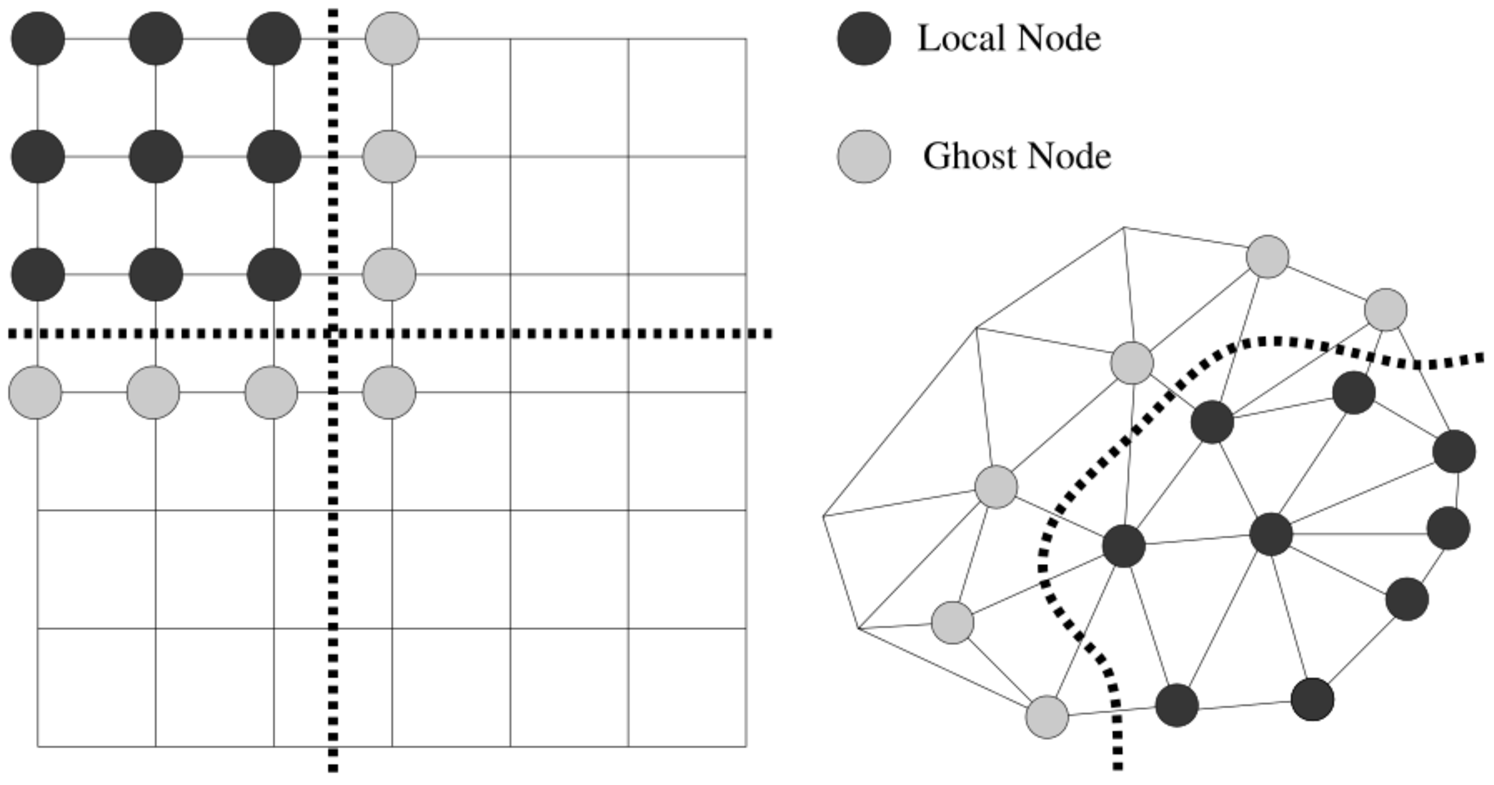
\includegraphics[width=0.9\textwidth]{petscghostvalues}
\caption{The standard \PETSc ghost figure, from }
\label{fig:petscghostvalues}
\end{figure}


\section{A finite difference method: assembling the linear system in parallel}

On the other hand, by a well-known Taylor's theorem argument \citep{MortonMayers}, for any function $F(x)$ which is sufficiently smooth,
    $$F''(x) = \frac{F(x+h) - 2 F(x) + F(x-h)}{h^2} + O(h^2)$$
as $h$ goes to zero.  To apply this formula to approximating the Laplacian in problem \eqref{poissonsquare}, we let $U_{i,j}$ be the approximation (which we compute) to the exact value $u(x_i,y_j)$ (which we don't suppose to know) of the solution $u$.  Also we denote $f_{i,j} = f(x_i,y_j)$.  Then we have this FD approximation to problem \eqref{poissonsquare}:
\begin{equation}
- \frac{U_{i+1,j} - 2 U_{i,j} + U_{i-1,j}}{h_x^2} - \frac{U_{i,j+1} - 2 U_{i,j} + U_{i,j-1}}{h_y^2} = f_{i,j}. \label{poissonsquareFD}
\end{equation}
Equation \eqref{poissonsquareFD} applies for all of the interior points where $1 \le i \le M-2$ and $1 \le j \le N-2$.  The boundary conditions in \eqref{poissonsquare} become $U_{0,j} = U_{M-1,j} = U_{i,0} = U_{i,N-1} = 0$, for all $i,j$.

Problem \eqref{poissonsquareFD} is a linear system.  We choose to treat all $MN$ locations on the grid as unknowns. FIXME: BUILD MATRIX, COMMENTING ON ROW SCALING (i.e. mult by $h_x h_y$ to improve conditioning)


\begin{marginfigure}
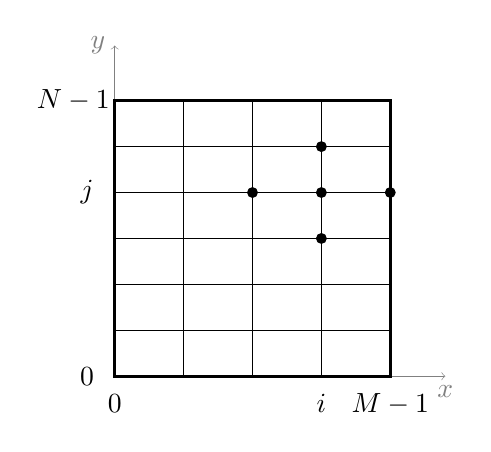
\begin{tikzpicture}[scale=3.5]
  \draw[->,gray,very thin] (0.0,0.0) -- (1.2,0.0) node[below] {$x$};
  \draw[->,gray,very thin] (0.0,0.0) -- (0.0,1.2) node[left] {$y$};
  \draw[line width=1.0pt] (0.0,0.0) -- (0.0,1.0) -- (1.0,1.0) -- (1.0,0.0) -- cycle;
  \node at (0.0,-0.1) {$0$};
  \node at (0.75,-0.1) {$i$};
  \node at (1.0,-0.1) {$M-1$};
  \node at (-0.1,0.0) {$0$};
  \node at (-0.1,0.666667) {$j$};
  \node at (-0.15,1.0) {$N-1$};
  \filldraw (0.50,0.666667) circle (0.5pt);
  \filldraw (0.75,0.666667) circle (0.5pt);
  \filldraw (1.00,0.666667) circle (0.5pt);
  \filldraw (0.75,0.5) circle (0.5pt);
  \filldraw (0.75,0.833333) circle (0.5pt);
  \draw[xstep=0.25,ystep=0.166667,black,thin] (0.0,0.0) grid (1.0,1.0);
\end{tikzpicture}
\caption{A stencil is shown on the grid at $i=3$ and $j=4$.}
\label{fig:unitsquaregridstencil}
\end{marginfigure}

\cinput{structuredlaplacian.c}{Fill matrix entries using \texttt{MatSetValuesStencil}.}{//CREATEMATRIX}{//ENDCREATEMATRIX}{code:structuredlaplacian}

\cinputpart{c2poisson.c}{The right side of equation \eqref{poissongridsystem} comes from differentiating the exact solution, which this method also computes.}{I}{//RHS}{//ENDRHS}{code:ctwopoissonrhs}

\cinputpart{c2poisson.c}{Set up \pDMDA \texttt{da} and \pMat \texttt{A} objects, and assemble the latter by calling \texttt{formlaplacian()}.}{II}{//CREATE}{//ENDCREATE}{code:ctwopoissoncreate}

\cinputpart{c2poisson.c}{Solve using \pKSP, and report on solution.}{III}{//SOLVE}{//ENDSOLVE}{code:ctwopoissonsolve}

\section{Runtime control of linear solver}

FIXME: basic Krylov theory

\section{Time-dependent heat equation}

FIXME: we WON'T do explicit, but it would look like ...

FIXME: use TS for backward-euler
